\documentclass[]{aa}

\usepackage{txfonts}
\usepackage[colorlinks, breaklinks]{hyperref}
\hypersetup{linkcolor=blue, citecolor=blue, filecolor=black, urlcolor=blue}

\usepackage{graphicx}
\graphicspath{{Article_figures/}{General_figures/}}

\usepackage{booktabs}
\usepackage{siunitx}
\usepackage[svgnames, dvipsnames, table]{xcolor}

\newcommand{\orcid}[1]{
\href{https://orcid.org/#1}{

\includegraphics[height=11pt]{ORCIDiD_icon128x128.png}}}

\newcommand{\snana}{\texttt{SNANA}}
\newcommand{\NN}[1]{\textcolor{orange}{#1}}

\newcommand{\prob}[2]{\mathcal{P}\left(#1 \mid #2\right)}

\begin{document}

\title{Implementation of the redshift evolution of type Ia supernovae in
SNANA}

\titlerunning{Implementation of the redshift evolution of type Ia supernovae in
SNANA}
\authorrunning{N.~Nicolas et al.}

\author{
    N. Nicolas\thanks{n.nicolas@ip2i.in2p3.fr, equal contribution} \inst{1} 
    \orcid{0000-0002-2681-6580}
    \and M. Rigault\thanks{m.rigault@ip2i.in2p3.fr, equal contribution} \inst{1}
    \orcid{0000-0002-8121-2560}
    \and M. Smith\inst{1,2}
    \and D. Scolnic\inst{3}
    \and B. Popovic\inst{3}
    \and\\ G. Aldering\inst{4}
    \and M. Briday\inst{1}
    \and Y. Copin \inst{1}
    \orcid{0000-0002-5317-7518}
    \and J. Lezmy \inst{1}
    \and J. Nordin\inst{5}
    \and Saul Perlmutter\inst{4}
    \orcid{0000-0002-3321-1432}
}

\institute{Univ Lyon, Univ Claude Bernard Lyon 1, CNRS, IP2I Lyon / IN2P3, IMR
    5822, F-69622, Villeurbanne, France
    \and
    University of Southampton, Southampton, UK
    \and
    Duke University, FILL IN AFFILIATION
    \and
    Physics Division, Lawrence Berkeley National Laboratory, 
    1 Cyclotron Road, Berkeley, CA, 94720, USA
    \and
    Institut fur Physik, Humboldt-Universität zu Berlin, Newtonstr. 15,
    12489 Berlin, Germany
}

\date{Submitted to A\&A\ the 19th of May 2020 / Accepted 26 February 2021}

\abstract{The use of Type Ia supernovae (SNe~Ia) as standard candles lead to a
    huge improvement on the constraints on cosmological parameters. In order to
    continue refining these values in a era of increasingly bigger datasets,
    systematic uncertainties have to be dealt with. Following previous work on
    the link between supernovae and their environment, we aim at finding the
    precise impact of a redshift-evolving underlying stretch distribution of
    SNe~Ia compared to the currently-used distributions in cosmological tool
\snana. We reproduced previous studies of the BBC team, then modified the
underlying stretch distribution and implemented an age step that logically
follows the use of an age-evolving population. We find that WHAT}

\keywords{Cosmology -- Type Ia Supernova -- Systematic uncertainties}
\maketitle

\section{Introduction}
\textit{General talk about SNe Ia, Hubble diagram, constraints and assumptions
from BBC to fit HD.}

Standardizing SNe Ia led to the discovery of the acceleration of the Universe's
expansion (\textbf{Riess98, Perlmutter99}): thanks to their color ($c$) and
stretch ($x_1$) parameters, the systematic uncertainty on their absolute
magnitude and thus their distance were greatly reduced. Dark energy is commonly
thought to be the cause of this expansion, and its equation-of-state parameter,
$w$, is currently know down to $\approx$ 4\% by combining constraints from both
SNe Ia and the Cosmic Microwave Background (\textbf{Scolnic18, Jones18,
Brout19b}). With the current effort to lower statistical uncertainties, the
systematic uncertainties are gaining in importance in the total error budget and
need to be addressed.

With that goal in mind, some recent studies try to improve the known
correlations. In \textbf{NR21}, we presented an initial study of the drift of
the underlying SNe~Ia stretch distribution as the function of redshift. We based
this study on the assumption of two populations of SNe~Ia, young and old, and
implemented different modelings of their distributions to better represent the
observed data. For that end we took SNe~Ia data and created a complete sample by
applying redshift cuts corresponding to the expected distance where no selection
effects should impact each survey. This approach was at the time the simplest
one to implement but does not allow to ponder the impact such a modeling has on
the cosmology, and mainly on $w$, and skips all selection effects altogether.

Other studies tend to define and refine other correlations between a SN's
brightness and some observable properties, such as their host-galaxy's mass
(\textbf{Sullivan10, Betoule14, Smith20}) or Star Formation Rate
(\textbf{Uddin17, Kim18, Rigault20}). One of the most common ways to test these
correlations is to use simulations (\textbf{Kessler09a, Scolnic18, Brout19}).
The SuperNova ANAlysis package (\snana, \textbf{Kessler09b}) allows to simulate
surveys by using underlying distributions of parameters and correlations between
them with the aim to find which ones come closest to the actual data.
\textbf{Scolnic \& Kessler 16} describes the procedure of finding these
distributions, implementing accurate selection effects for each survey, noise
and intrinsic scatter that shift them to the observed distributions. In this
framework, it's a galaxy's stellar mass ($M_\mathrm{stellar}$) that is assumed
as the main observable responsible for its environmental effects on SNe~Ia. The
goal is to correct the values of SNe affected by Malmquist bias by computing the
average of the simulated ones, as opposed to our first approach of getting rid
of the affected SNe.

These simulated surveys have been used to study the dependence with redshift of
the bias correction (\textbf{Kessler 09a, Betoule14}), but showed remnant
correlations in the computed distance moduli (SK16). The analysis thus went from
1-dimensional to a 5-dimensional parameter space, studying the correlations with
redshift, color, stretch, color-luminosity and stretch-luminosity relationship
parameters ($\alpha$, $\beta$) as developed by \textbf{Kessler \& Scolnic 17}
with the BEAMS with Bias Corrections (BBC) method, hereafter refered to as
BBC5D. This method is used in both the Dark Energy Survey 3 years (DES3YR,
\textbf{Abbott19, Brout19b}) and Panoramic Survey Telescope and Rapid Response
System (PAN-STARRS, \textbf{Scolnic18, Jones18}) analyses. This formalism was
further improved based on the work of \textbf{Smith20}

\section{Modeling}\label{sec:model}

In our first analysis, we based our work on a two-populations modeling based on
age: a young ($\log(\mathrm{LsSFR}) \geq -10.82$) and an old one
($\log(\mathrm{LsSFR}) < -10.82$). We determined the underlying stretch
distribution for both these populations, and used the evolution of the fraction
of young SNe~Ia given by
\begin{equation}\label{eq:delta}
    \delta(z) = \left(K^{-1}\times\left(1+z\right)^{-2.8}+1\right)^{-1} 
\end{equation}
we determined a relationship between SNe~Ia stretches and redshift. Supposing
age is the driving phenomenon behind the different systematics seen in SNe~Ia
cosmology also implies that SNe~Ia have an age step of $0.130\,\mathrm{mag}$
rather than a mass step of $0.050\,\mathrm{mag}$. In this work we are trying to
generate simulations to ponder the impact of these systematics on the
determination of cosmological parameters, and notably $w$.

In order to simulate SNe, we require a host galaxy to follow the distributions
of what has been observed by the different simulated surveys. While we argue
that LsSFR is a better tracer of a SN's environment (\textbf{Briday 21}), most
survey characterize galaxies using their stellar mass. Therefore, to compare the
implication of our modeling based on LsSFR with what other surveys observed, we
need to modelize galaxy masses with respect to LsSFR using the same sample as
described in Section 2 of \textbf{NR21}.

\subsection{Modeling the mass}
Following \textbf{NR21}, we use the LsSFR as the tracer of the age of a SN on
the mass estimates from SNf, then model the young and old population through a
series of different parameterizations and pick the lowest AIC one. However, SNf
masses were computed using Eq. 8 of \textbf{Taylor 2011} (see \textbf{Rigault
20}) while other surveys from the Pantheon catalog use different techniques of
mass estimation that might give different output values for a same galaxy. The
estimate from Taylor involves the absolute $i$-band AB-magnitude $M_i$. It is
deduced from the apparent magnitude $m_i$ knowing the galaxy's redshift but
assumes that the observed $i$ band is close to the restframe one, which is true
for the SNf redshifts which are below $z~0.05$. Surveys from the Pantheon sample
are at higher redshifts and used SED to avoid K-corrections in that procedure.
In order to maintain coherence between the mass modeling based on SNf data and
the masses measured in the Pantheon surveys we will simulate, we needed to use
the same method for each object. We thus chose to use SED fitting for everyone.

\textbf{A few words about SED fitting}

Based on the shape of the $M_{\rm host}$ vs LsSFR scatter plot, different
modelings were implemented. There are referred to by the number of Gaussian
functions, Mean values and Sigma values that compose their mathematical
behavior. For instance, a modeling having 1 symmetric Gaussian with different
means for each population is labeled 2G2M2S. A total of 8 modelings have been
tested for this study:

\begin{itemize}
    \item 1G1M1S also simply named \textit{Gaussian}, a pure
        redshift-independent and age-independent Gaussian modeling;

    \item 1G1M2S or \textit{Asymmetric}, using a unique asymmetric Gaussian;

    \item 2G2M2S or \textit{Howell}, based on the work from \textbf{HOWELL07}
        and previously described;

    \item 2G2M3S with one Gaussian for the young population and one asymmetric
        Gaussian for the old one;

    \item 2G2M4S or \textit{Asymmetric Howell} with one asymmetric Gaussian per
        population;

    \item 3G3M3S or \textit{Free Base}, close to the base model of \textbf{NR21}
        with a single Gaussian for the young population and a Gaussian mixture
        for the old population, each having a different mean;

    \item 3G3M4S using Free Base with a mixture of Gaussian and asymmetric
        Gaussian;

    \item 4G4M4S or \textit{Double Howell}, having one Gaussian mixture for each
        population.
\end{itemize}

\subsection{Mass modeling results}

Each one of these modelings is adjusted on the whole Pantheon dataset,
following the procedure in Section 3 of \textbf{NR21} depending on the presence
of LsSFR measurments in each sub-survey. The results are gathered in Table
\ref{tab:modelcomp} where 
\begin{equation}\label{eq:likelihood}
    -2\ln(L) = -2 \sum_i \ln \prob{x_1^i}{\vec{\theta};
    \mathrm{d}x_1^i, y^i}.
\end{equation}
and 
\begin{equation}
    \mathrm{AIC} = -2\ln(L) + 2k,
\end{equation}

Due to unrealistically small errors on the last three modelings thus holding no
physical meaning, we discarded them in the analysis regardless of their fitting
quality. We used the Akaike Information Criterion (AIC, \textbf{BURNHAM01}) to
compare each model's ability to properly describe the observations, penalizing
additionnal degrees of freedom to avoid overfitting the data. After computation,
the best, lowest-AIC model is the Asymmetric Howell modeling, in which the mass
distribution of the younger population ($\log(\mathrm{LsSFR}) \geq -10.82$) and
the older population ($\log(\mathrm{LsSFR}) < -10.82$) are modeled as asymmetric
Gaussians $\mathcal{N}\left(\mu, \sigma_{-\mathrm{y,o}}^2\; \text{if}
\;x_1<\mu,\; \text{else} \;\sigma_{+\mathrm{y,o}}^2\right)$. A graphical
representation is shown Fig. \ref{fig:massmodel}. The parameters value we found
are summarized Table \ref{tab:modelresults}.

\begin{figure}[]
    \centering
    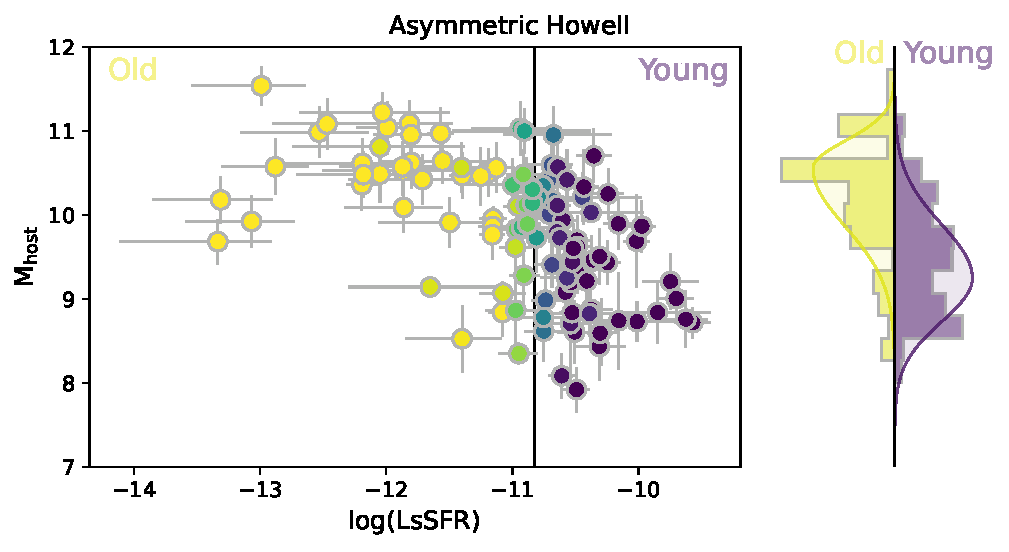
\includegraphics[width=\linewidth]{model_mass_2G2M4S_hist_SED-nonan.pdf}
    \caption{\textit{Main}: SED-fitted host mass ($M_\mathrm{host}$) as a
        function of the LsSFR for SNfactory SNe. The color corresponds to the
        probability, $p_y$, for the SNe~Ia to be young, i.e., to have
        $\log\mathrm{LsSFR} \geq -10.82$ \citep[see][]{rigault2020}.
    \textit{Right}: $p_y$-weighted histogram of the SN masses, as well as the
adjusted model; contributions of the younger and older population are shown in
purple and yellow, respectively.}
    \label{fig:massmodel}
\end{figure}

\begin{table*}
    \centering
    \caption{Comparison of the relative ability of each model to describe the
        data. For each considered model, we report whether the model is
        drifting, its number of free parameters, $-2\ln(L)$ (see
        Eq.~\ref{eq:likelihood}), the AIC and the AIC difference ($\Delta$AIC)
        between this model and the base model used as reference because it has
    the lowest AIC.}
    \label{tab:modelcomp}
    \begin{tabular}{lcccccccc}
        %\hline\hline & & & & & & \\[-0.6em]
        \toprule
        & & & \multicolumn{3}{c}{Fiducial sample (569 SNe)}
            & \multicolumn{3}{c}{Conservative sample (422 SNe)} \\
        \cmidrule(lr){4-6}\cmidrule(lr){7-9}
        Name & drift & $k$ &
        $-2\ln(L)$ & AIC & $\Delta$AIC & $-2\ln(L)$ & AIC & $\Delta$AIC\\[0.2em]
        %\hline & & & & & & \\[-0.6em]
        \midrule

        Asym Howell & $\delta(z)$ & 6
        & 1538.7 & 1550.7 & -- 
        & 1197.4 & 1209.4 & -- \\

        Howell & $\delta(z)$ & 4
        & 1546.6 & 1554.6 & $-4.0$
        & 1205.0 & 1213.0 & $-3.6$ 
        \\

        Asym+Howell & $\delta(z)$ & 5
        & 1546.5 & 1556.5 & $-5.8$
        & 1204.8 & 1214.8 & $-5.4$ 
        \\

        Asymmetric & -- & 3
        & 1593.1 & 1599.1 & $-48.5$
        & 1248.6 & 1254.6 & $-45.2$ 
        \\

        Gaussian & -- & 2
        & 1608.3 & 1612.3 & $-61.6$
        & 1258.2 & 1262.2 & $-52.8$ 
        \\
        \bottomrule
    \end{tabular}
\end{table*}

\begin{table*}
    \centering
    \caption{Best-fit values of the parameters for the mass distribution
    model when applied to the SNfactory dataset only (114 SNe~Ia).}
    \label{tab:modelresults}
    \begin{tabular}{lcccccc}
        %\hline\hline & & & & & & \\[-0.6em]
        \toprule
        Sample  & $\mu_\mathrm{y} $ &
                $\sigma_{-,\mathrm{y}}$ & $\sigma_{+,\mathrm{y}}$
                & $\mu_\mathrm{o} $ &
                $\sigma_{-,\mathrm{o}}$ & $\sigma_{+,\mathrm{o}}$ \\[0.2em]
        %\hline & & & & & & \\[-0.4em]
        \midrule
        SNFactory     & $ 9.34 \pm 0.10 $
                      & $0.51 \pm 0.07 $ & $0.95 \pm 0.07 $
                      & $10.74 \pm 0.48 $
                      & $ 0.48 \pm 0.06 $ & $0.39 \pm 0.06 $ \\
        Fiducial      & $ 9.34 \pm 0.10 $
                      & $0.51 \pm 0.07 $ & $0.95 \pm 0.07 $
                      & $10.74 \pm 0.48 $
                      & $ 0.48 \pm 0.06 $ & $0.39 \pm 0.06 $ \\
        Conservative  & $ 9.23 \pm 0.10 $
                      & $0.47 \pm 0.07 $ & $0.96 \pm 0.07 $
                      & $10.61 \pm 0.48 $
                      & $ 0.41 \pm 0.06 $ & $0.44 \pm 0.06 $ \\
        \bottomrule
    \end{tabular}
\end{table*}

\section{SNANA}

SNANA is a combination of tools to simulate SNe Ia data and exploit these to put
constraints on cosmological parameters by fitting a Hubble diagram with them.
There are 3 main parts to this procedure: (1) generate a lightcurve by modeling
a SN and how each survey would acquire it, taking selection effects into
account; (2) fit said lightcurve with \texttt{SALT2.4} and extract the $m_b$,
$x_1$, $c$ and $t_0$ parameters; (3) infer distance modulus values using bias
correction.

These tools begin by generating a Spectral Energy Distribution to which are
applied astrophyical effects such as lensing, dimming, redshifting or galactic
extinction, giving a first simulated magnitude. Then this magnitude is converted
into an observed one (flux) by reproducing the effects of the instruments: zero
point, sky noise and PSF. Selection effects are finally applied to mimick the
triggering of which events are analyzed; these include the needed number of
detections and needed band(s) and the spectroscopic efficiency function of the
simulated surveys. This leads to simulated lightcurves, and after a
\texttt{SALT2.4} fit we can get to distance modulus values following the BBC
framwork from \textbf{KS17}, which is defined as:

\begin{equation}\label{eq:mu}
    \mu = m_B + \alpha x_1 - \beta c - M_{z_i} + \delta\mu _\mathrm{host} +
    \delta\mu _\mathrm{bias}
\end{equation}

\subsection{Environmental impact and HOSTLIB}
However, the definition of a realistic model is the be questioned. In the
pioneer work of \textbf{SK16}, there were no relationship between SNe and their
host galaxy. \textbf{P21} and \textbf{M20} introduced a link between the two
thanks to a HOSTLIB: a table of 100,000 galaxies made to mimic the actual
surveyed galaxies by the different samples. To each galaxy is associated a SN
through its main fitted properties such as $x_1$ or $c$, which are generated by
models of underlying distributions. Yet, this process was directed at guessing
what relationship would fit more the data, by using bins of host galaxy masses
and minimizing asymmetric Gaussian distributions for each in a backward-modeling
way. It's a non-direct method to infer an evolution of an underlying
distribution as a function of mass.

Our approach was to use independent data from the SNf sample that uses LsSFR to
characterize a galaxy, as explained in Section \ref{sec:model}, and make an
evolving, analytical model that can then describe higher-redshift SNe in a
forward-modeling approach. This method has the aim to be predictive and to
better fit the data, as is discussed in Section \ref{sec:results}. In order to
implement our modeling in this framework, we had to modify the HOSTLIBs on which
the simulations are based.

\subsection{Input generation}\label{ssec:inpgen}

Having the two modelings for mass and stretch allows us to pick a redshift and
generate a mass and a stretch value. This will in turn give us the ability to
match the HOSTLIB's masses and replace the stretch values by our \textbf{N21}
modeling's predictions. This is done with the \textit{SNprop} Python
module\footnotemark \footnotetext{https://github.com/MickaelRigault/snprop}.
Given a redshift or lists of redshift, it takes the expected fraction of young
stars using $\delta(z)$ from Eq.~\ref{eq:delta} then sets a ``young'' or ``old''
flag by picking a random value $r$ between 0 and 1 and comparing it to said
fraction. If $r < \delta(z)$, then the simulated SN will be young and
conversely. The higher the $z$, the higher the $\delta(z)$, and thus the higher
the probability to flag it young. A graphical explanation is given
Fig.~\ref{fig:deltaz}. Stretch and mass values are then generated with the
previous modelings depending whether the progenitor is considered young or old.

\begin{figure}[]
    \centering
    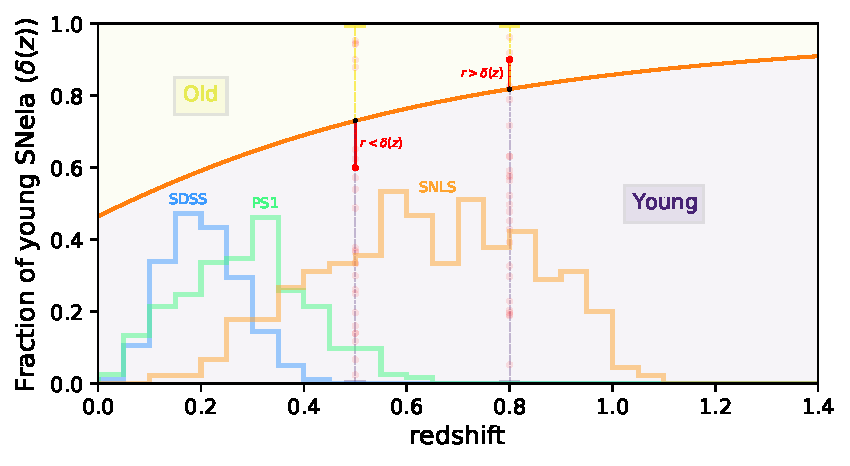
\includegraphics[width=\linewidth]{deltaz_hist_yo-random.pdf}
    \caption{\textit{Orange}: Estimated fraction of young SNe as a function of
        redshift. \textit{Histograms}: Number of SNe in bins of redshift for the
        3 main surveys of the Pantheon sample, not scaled. \textit{Red vertical
        lines}: For each $z$, a random number $a$ between 0 and 1 is picked: if
    it's lower (higher) than $\delta(z)$ at that redshift then the SN will be
young (old), and the distributions of mass and stretch to pick from will follow
this flag.}
    \label{fig:deltaz}
\end{figure}


% SK16 is galaxy distribution from which you draw, P21 is a list with the
% distrubtion already in it, linking the relationships and $x_1$ and stuff
% already drawn. But there's no evolution in it, and we want to do that. Forward
% model that through.

% General, Brodie, us; no lightcurve fitting, and at the end of hostlib section
% w simulate antheon

% P21: There is a relationship, we'll try to guess it. Take data bns of mass,
% and calculate what the distribtion of stretch is for each. Looks differently
% in different bins: as a function of mass they have distribution. Backward
% models.  N21: our data is independent and we use it to show that it works on
% other data at higher redshift, is predictive, and involves an evolution of the
% distributions.

% Generate $z$, take closest $M$ entry in a table of host galaxies (HOSTLIB),
% then pick $x_1$, $c$ assuming underlying relationships defined by the BBC
% team.  Because we want to make these simulations with an evolving underlying
% distribution, we have to replace then $x_1$ values by what is estimated by our
% previous model.

% Section 3

% Having mass isn't constitutive of SNANA, not a requirment, but we use it
% because the actual data we compare our simulated data to is described using
% mass. So we need a link betwwen LsSFR to mass: high-redshift galaxies only
% have mass measurments, not LsSFR. Quote Martin's paper.

% given model and observation strategy, what do you see like SIMSURVEY.

% SImulation part of SNANA separate from distance.

\section{Results of modeling}\label{sec:results}
In order to see the impact of our modeling in the inferred $w$ value, we first
needed to get on-par with the current best work on that matter, working closely
with the SNANA team to recreate the results of \textbf{P21} before using our
HOSTLIB.

\subsection{Description of the tests}\label{ssec:kinds}
We defined 4 ways to simulate SNe depending on the assumptions that can be made.
First, ``SK'' based on \textbf{SK16} where there are no link between a SN and
its host galaxy (in practice using a HOSTLIB without taking the additionnal
correlations into account). Then, ``BP'' based on \textbf{P21} where the $x_1$
and $c$ parameters of the HOSTLIB are generated by asymmetric Gaussian modelings
adjusted to reproduce the observed distributions in nature. The first new
HOSTLIB, dubbed ``NN'', is based on BP but replacing the $x_1$ values following
the previously described procedure, effectively adding one of the consequences
of supposing age as the leading factor between SNe and their environment. The
second new HOSTLIB is dubbed ``NR'', but adds an age column defined by
$\mathrm{age} = \left\{
    \begin{array}{l}
        0 \quad \mathrm{if} \quad r < \delta(z)\\
        1 \quad \mathrm{if} \quad r > \delta(z)
    \end{array}
\right.$ as discussed in Section~\ref{ssec:inpgen}, and an step column in which
we associate a step of $\pm0.065\,\mathrm{mag}$ for young and old SNe
respectively. This step value stems from the other implication of age as the
driving phenomenon under the SNe~Ia correlations, defined in \textbf{R21? B21?}.

In order to replicate the actual datasets on which our stretch model was based
on, i.e. the Pantheon dataset \NN{what do we do of LOWZ?}, we implemented two
approaches of simulation:

\begin{enumerate}
    \item using one DATA sample with (FIND NUMBER) SNe and a unique huge BIASCOR
        sample of (FIND NUMBER), simulations stamped ``FULL'' hereafter;
    \item and a collection of 500 already sample-sized DATA samples that are
        each corrected with the same BIASCOR sample.
\end{enumerate} 

For each of them, finding the scaling factor of NGEN (describe) for each survey
proved crucial to the study. They were computed to have approximately the same
ratio of DATA between surveys at the end of the fitting stage than in Pantheon,
that is shown Table~\ref{tab:ratio}.

\begin{table}
    \centering
    \caption{Number of data in Pantheon and relative ratio with respect to the
    smallest sample, LOWZ}
    \label{tab:ratio}
    \begin{tabular}{lcc}
        \toprule
        Survey & Number & Ratio/LOWZ \\
        \midrule
        LOWZ   & 172    & 1.00 \\
        SDSS   & 335    & 1.95 \\
        PS1    & 279    & 1.62 \\
        SNLS   & 236    & 1.37 \\
        \bottomrule
    \end{tabular}
\end{table}

\NN{Melting pot of things to talk about, maybe some in appendix:
\begin{itemize}
    \item Different HOSTLIBs depending on the survey (lowz, highz);
    \item Plot HOSTLIBs parameters
    \item Weigthmaps, plot them
    \item Talk about NGENs and how they are made to fit to the ratio in Pantheon
        \begin{itemize}
            \item Check differences between NN/NR and SK/BP
            \item It might be that having to up the NGENs of non-LOWZ surveys in
                NN/NR wrt SK/BP while keeping LOWZ's NGEN to 20.0 could be a
                result about the impact of this modeling on the generated number
                of low redshift SNe
        \end{itemize}
    \item Inputs:
        \begin{itemize}
            \item $H_0 = \SI{70.0}{km.s^{-1}.Mpc^{-1}}$
            \item $\alpha = 0.145$;
            \item $\beta = 3.1$;
            \item $w = -1$;
            \item $\Omega_m = 0.315$;
            \item $\Omega_\Lambda = 0.685$
        \end{itemize}
    \item Spectroscopic efficiencies
    \item In inputs:
        \begin{itemize}
            \item GENMODEL: SALT2.JLA-B14 for all but LOWZ: SALT2.WFIRST-H17
            \item Intrinsic scatter: G10
            \item SNR > 4 or 2
            \item CUTWIN\_NEPOCH = 5 -5
            \item GENFILTERS? GENRANGE\_REDSHIFT?
            \item GENMEAN, RANGE, SIGMA for x1, c, alpha beta?
        \end{itemize}
    \item For LCFIT stage, SNRMAX = 5 for LOWZ, not the others, beware
        cosmological parameters in that stage
    \item Role of biascor samples
    \item Flavors of biascor samples:
        \begin{itemize}
            \item 1D
            \item 5D
            \item 7D
        \end{itemize}
\end{itemize}}

\subsection{Comparing tests on simulations}
Before comparing the $w$ v $\Omega_m$ values, we looked at the correspondence
between simulated data and actual data to ensure the improvement of our
LsSFR-based approach. The main idea being the evolution of the underlying stretch
distribution as a function of redshift, we represented $x_1$ v $z$ in log-scale
using a 2D hexagonal colored histogram for the simulated data and dots for the
Pantheon values. We also looked at the $x_1$ v $M\mathrm{host}$ plot to ponder
the relationship these two main characteristics of the SNe~Ia on one hand and the
host galaxies on the other (see \ref{fig:P21vN21}). We then computed a 2D kernel
of each set of parameters based on the simulations and determined the associated
$\chi^2$ between the data and the kernels. The results are summarized in Table
\ref{tab:chi2comp} and the code in the \textit{SNprop} module.

\begin{figure*}
    \centering
    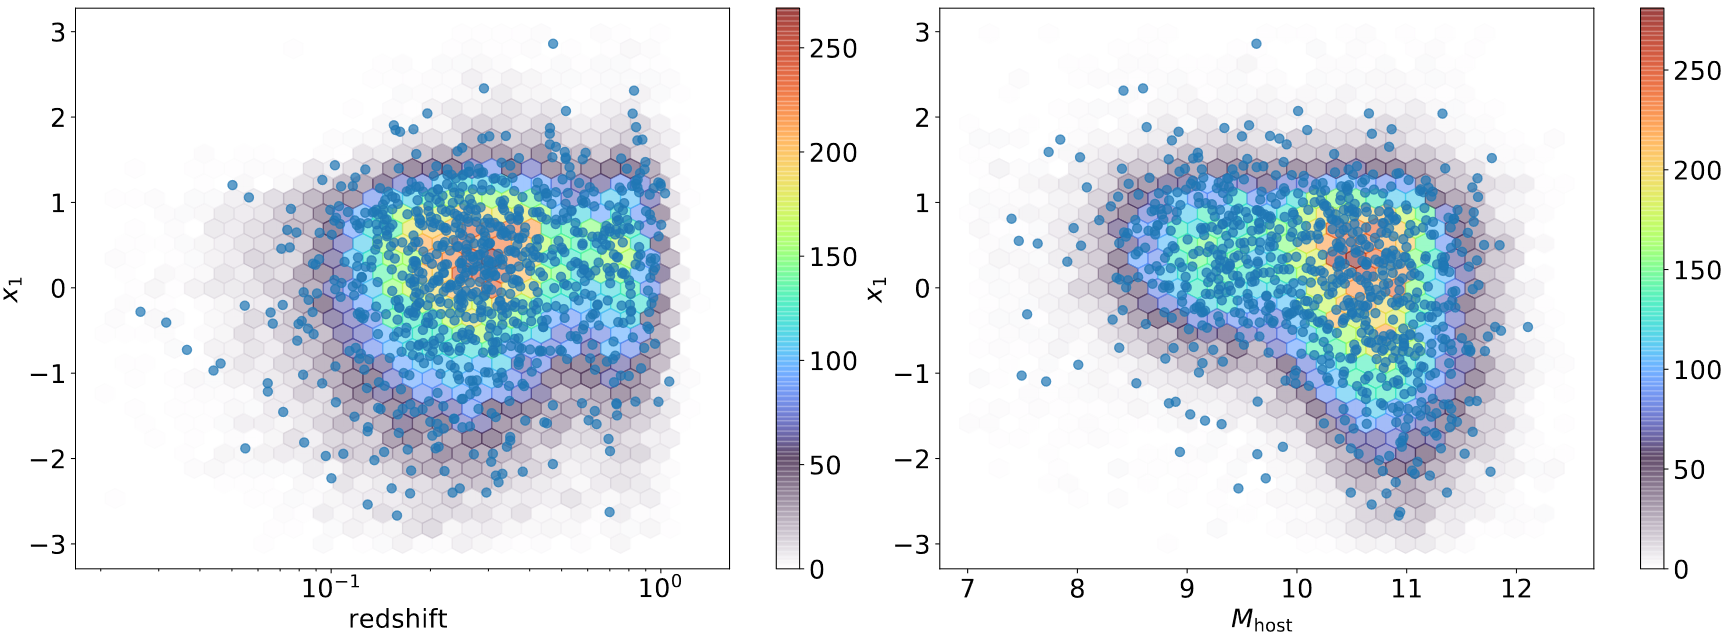
\includegraphics[width=\linewidth]{kernel-compare.png}
    \caption{\textit{Top}: 2D hexagonal histograms of the simulated data using
    the P21 setup in color (left: $x_1$ v $z$, right: $x_1$ v $M_\mathrm{host}$)
    and actual Pantheon data in blue points. \textit{Bottom}: same data but
    2D hexagonal histograms of the simulated program using the N21 improved
    HOSTLIB.}
    \label{fig:P21vN21}
\end{figure*}

\begin{table}
    \centering
    \caption{Comparison of the relative ability of each HOSTLIB implementation
    to describe the data. For each HOSTLIB a 2D KDE is computed from the simulated
    data and used to determine said $\chi^2$.}
    \label{tab:comp}
    \begin{tabular}{c|cc}
        \hline\hline
                & \multicolumn{2}{c}{$\chi^2$}
        \\
        HOSTLIB & $x_1$ v $z$ & $x_1$ v $M_\mathrm{host}$
        \\\hline
        P21     & ????        & ????
        \\
        N21     & ????        & ????
        \\
        \hline
    \end{tabular}
\end{table}

The numerical values follow what was already clear on the figures: it fits best.

\section{Impact on cosmology}
What we want is not so much $w$ than $\Delta w$ wrt. best current work. We find
x\% and here are the contours.

\section{Discussion}\label{sec:discussion}
We expected to have a higher/lower, and we got that.

\section{Conclusion}\label{sec:ccl}

Should be nice.

\begin{acknowledgements}
    This project has received funding from the European Research Council (ERC)
    under the European Union's Horizon 2020 Research and Innovation program
    (grant agreement no 759194 - USNAC).
    This work was supported in part by the Director, Office of Science, Office
    of High Energy Physics of the U.S. Department of Energy under Contract No.
    DE-AC025CH11231.
    This project is partly financially supported by Région Rhône-Alpes-Auvergne.
\end{acknowledgements}

\end{document}
\bibliographystyle{aa}
\begin{thebibliography}{} 
% A

\bibitem[Abbott et al.(2019)]{descosmopaper2019} Abbott, T.~M.~C., Allam, S.,
Andersen, P., et al.\ 2019, \apjl, 872, L30

\bibitem[Aldering et al.(2002)]{aldering2002} Aldering, G., Adam, G., Antilogus,
P., et al.\ 2002, \procspie, 61

\bibitem[Aldering et al.(2020)]{aldering2020} Aldering, G., Antilogus, P.,
Aragon, C., et al.\ 2020, Research Notes of the American Astronomical Society,
4, 63

\bibitem[Astier et al.(2006)]{astier2006} Astier, P., Guy, J., Regnault, N., et
al.\ 2006, \aap, 447, 31

\bibitem[Aubourg et al.(2008)]{aubourg2008} Aubourg, {\'E}., Tojeiro, R.,
Jimenez, R., et al.\ 2008, \aap, 492, 631 

% B

\bibitem[Bazin et al.(2011)]{bazin2011} Bazin, G., Ruhlmann-Kleider, V.,
Palanque-Delabrouille, N., et al.\ 2011, \aap, 534, A43

\bibitem[Bellm et al.(2019)]{bellm2019} Bellm, E.~C., Kulkarni, S.~R., Graham,
M.~J., et al.\ 2019, \pasp, 131, 018002

\bibitem[Betoule et al.(2014)]{betoule2014} Betoule, M., Kessler, R., Guy, J.,
et al.\ 2014, \aap, 568, A22

\bibitem[Burnham \& Anderson(2004)]{burnham2004} Burnham, K., Anderson, D., \
2004, Sociological Methods \& Research, 33, 2

% C

\bibitem[Campbell et al.(2013)]{campbell2013} Campbell, H., D'Andrea, C.~B.,
Nichol, R.~C., et al.\ 2013, \apj, 763, 88

\bibitem[Childress et al.(2013)]{childress2013} Childress, M., Aldering, G.,
Antilogus, P., et al.\ 2013, \apj, 770, 108

\bibitem[Childress et al.(2014)]{childress2014} Childress, M.~J., Wolf, C., \&
Zahid, H.~J.\ 2014, \mnras, 445, 1898

% D

\bibitem[D'Andrea et al.(2011)]{dandrea2011} D'Andrea, C.~B., Gupta, R.~R.,
Sako, M., et al.\ 2011, \apj, 743, 172

\bibitem[Dilday et al.(2008)]{dilday2008} Dilday, B., Kessler, R., Frieman,
J.~A., et al.\ 2008, \apj, 682, 262

% E
% F

\bibitem[Feeney et al.(2019)]{feeney2019} Feeney, S.~M., Peiris, H.~V.,
Williamson, A.~R., et al.\ 2019, \prl, 122, 061105

\bibitem[Freedman et al.(2019)]{freedman2019} Freedman, W.~L., Madore, B.~F.,
Hatt, D., et al.\ 2019, \apj, 882, 34

\bibitem[Freedman et al.(2020)]{freedman2020} Freedman, W.~L., Madore, B.~F.,
Hoyt, T., et al.\ 2020, \apj, 891, 57. doi:10.3847/1538-4357/ab7339

\bibitem[Frieman et al.(2008)]{frieman2008} Frieman, J.~A., Bassett, B., Becker,
A., et al.\ 2008, \aj, 135, 338

% G

\bibitem[Graham et al.(2019)]{graham2019} Graham, M.~J., Kulkarni, S.~R., Bellm,
E.~C., et al.\ 2019, \pasp, 131, 078001

\bibitem[Gupta et al.(2011)]{gupta2011} Gupta, R.~R., D'Andrea, C.~B., Sako, M.,
et al.\ 2011, \apj, 740, 92

\bibitem[Guy et al.(2007)]{guy2007} Guy, J., Astier, P., Baumont, S., et al.\
2007, \aap, 466, 11

% H

\bibitem[Hamuy et al.(1996)]{hamuy1996} Hamuy, M., Phillips, M.~M., Suntzeff,
N.~B., et al.\ 1996, \aj, 112, 2391

\bibitem[Hamuy et al.(2000)]{hamuy2000} Hamuy, M., Trager, S.~C., Pinto, P.~A.,
et al.\ 2000, \aj, 120, 1479

\bibitem[Hinton et al.(2019)]{hinton2019} Hinton, S.~R., Davis, T.~M., Kim,
A.~G., et al.\ 2019, \apj, 876, 15

\bibitem[Howell et al.(2007)]{howell2007} Howell, D.~A., Sullivan, M., Conley,
A., et al.\ 2007, \apjl, 667, L37

% I

\bibitem[Ivezi{\'c} et al.(2019)]{lsstpaper} Ivezi{\'c}, {\v{Z}}., Kahn, S.~M.,
Tyson, J.~A., et al.\ 2019, \apj, 873, 111

% J

\bibitem[Jones et al.(2015)]{jones2015} Jones, D.~O., Riess, A.~G., \& Scolnic,
D.~M.\ 2015, \apj, 812, 3 1

\bibitem[Jones et al.(2019)]{jones2019} Jones, D.~O., Scolnic, D.~M., Foley,
R.~J., et al.\ 2019, \apj, 881, 19

% K

\bibitem[Kelly et al.(2010)]{kelly2010} Kelly, P.~L., Hicken, M., Burke, D.~L.,
et al.\ 2010, \apj, 715, 743

\bibitem[Kessler et al.(2009)]{kessler2009} Kessler, R., Becker, A.~C., Cinabro,
D., et al.\ 2009, \apjs, 185, 32

\bibitem[Kessler et al.(2009)]{SNANA} Kessler, R., Bernstein, J.~P., Cinabro,
D., et al.\ 2009, \pasp, 121, 1028

\bibitem[Kessler \& Scolnic(2017)]{kessler2017} Kessler, R., \& Scolnic, D.\
2017, \apj, 836, 56

\bibitem[Kim et al.(2018)]{kim18} Kim, Y.-L., Smith, M., Sullivan, M., et al.\
2018, \apj, 854, 24

\bibitem[Kim et al.(2019)]{kim19} Kim, Y.-L., Kang, Y., \& Lee, Y.-W.\ 2019,
Journal of Korean Astronomical Society, 52, 181

\bibitem[Knox \& Millea(2020)]{knox2019} Knox, L. \& Millea, M.\ 2020, \prd,
101, 043533. doi:10.1103/PhysRevD.101.043533

% L

\bibitem[Lampeitl et al.(2010)]{lampeitl2010} Lampeitl, H., Smith, M., Nichol,
R.~C., et al.\ 2010, \apj, 722, 566

% M

\bibitem[Mannucci et al.(2005)]{mannucci2005} Mannucci, F., Della Valle, M.,
Panagia, N., et al.\ 2005, \aap, 433, 807 

\bibitem[Mannucci et al.(2006)]{mannucci2006} Mannucci, F., Della Valle, M., \&
Panagia, N.\ 2006, \mnras, 370, 773 

\bibitem[Maoz et al.(2014)]{maozmannucci2014} Maoz, D., Mannucci, F., \&
Nelemans, G.\ 2014, \araa, 52, 107 


% N

\bibitem[Neill et al.(2006)]{neill2006} Neill, J.~D., Sullivan, M., Balam, D.,
et al.\ 2006, \aj, 132, 1126

\bibitem[Neill et al.(2009)]{neill2009} Neill, J.~D., Sullivan, M., Howell,
D.~A., et al.\ 2009, \apj, 707, 1449

\bibitem[Nordin et al.(2018)]{nordin2018} Nordin, J., Aldering, G., Antilogus,
P., et al.\ 2018, \aap, 614, A71

% O
% P

\bibitem[Pan et al.(2014)]{pan2014} Pan, Y.-C., Sullivan, M., Maguire, K., et
al.\ 2014, \mnras, 438, 1391

\bibitem[Perlmutter et al.(1999)]{perlmutter1999} Perlmutter, S., Aldering, G.,
Goldhaber, G., et al.\ 1999, \apj, 517, 565

\bibitem[Perrett et al.(2010)]{perrett2010} Perrett, K., Balam, D., Sullivan,
M., et al.\ 2010, \aj, 140, 518

\bibitem[Phillips(1993)]{phillips1993} Phillips, M.~M.\ 1993, \apjl, 413, L105

\bibitem[Planck Collaboration et al.(2020)]{planck2018} Planck
Collaboration, Aghanim, N., Akrami, Y., et al.\ 2020, \aap, 641, A6.
doi:10.1051/0004-6361/201833910

% Q
% R

\bibitem[Reid et al.(2019)]{reid2019} Reid, M.~J., Pesce, D.~W., \& Riess,
A.~G.\ 2019, \apjl, 886, L27. doi:10.3847/2041-8213/ab552d

\bibitem[Rest et al.(2014)]{rest2014} Rest, A., Scolnic, D., Foley, R.~J., et
al.\ 2014, \apj, 795, 44

\bibitem[Riess et al.(1998)]{riess1998} Riess, A.~G., Filippenko, A.~V.,
Challis, P., et al.\ 1998, \aj, 116, 1009

\bibitem[Riess et al.(2009)]{riess2009} Riess, A.~G., Macri, L., Casertano, S.,
et al.\ 2009, \apj, 699, 539

\bibitem[Riess et al.(2016)]{riess2016} Riess, A.~G., Macri, L.~M., Hoffmann,
S.~L., et al.\ 2016, \apj, 826, 56

\bibitem[Riess et al.(2018)]{riess2018} Riess, A.~G., Casertano, S., Yuan, W.,
et al.\ 2018, \apj, 861, 126

\bibitem[Riess et al.(2019)]{riess2019} Riess, A.~G., Casertano, S., Yuan, W.,
et al.\ 2019, \apj, 876, 85

\bibitem[{Rigault et al.(2013)}]{rigault2013} Rigault, M., Copin, Y.,
Aldering, G., {et~al.} 2013, \aap, 560, A66

\bibitem[Rigault et al.(2015)]{rigault2015} Rigault, M., Aldering, G., Kowalski,
M., et al.\ 2015, \apj, 802, 20

\bibitem[Rigault et al.(2020)]{rigault2020} Rigault, M., Brinnel, V., Aldering,
G., et al.\ 2020, \aap, 644, A176

\bibitem[Rodney et al.(2014)]{rodney2014} Rodney, S.~A., Riess, A.~G., Strolger,
L.-G., et al.\ 2014, \aj, 148, 13 
  
\bibitem[Roman et al.(2018)]{roman2018} Roman, M., Hardin, D., Betoule, M., et
al.\ 2018, \aap, 615, A68

\bibitem[Rose et al.(2019)]{rose2019} Rose, B.~M., Garnavich, P.~M., \& Berg,
M.~A.\ 2019, \apj, 874, 32

\bibitem[Rubin et al.(2015)]{rubin2015} Rubin, D., Aldering, G., Barbary, K., et
al.\ 2015, \apj, 813, 137

\bibitem[Rubin \& Hayden(2016)]{rubin2016} Rubin, D., \& Hayden, B.\ 2016,
\apjl, 833, L30

% S

\bibitem[Sako et al.(2008)]{sako,2008} Sako, M., Bassett, B., Becker, A., et al.\
2008, \aj, 135, 348

\bibitem[Scannapieco \& Bildsten(2005)]{scannapieco,2005} Scannapieco, E., \&
Bildsten, L.\ 2005, \apjl, 629, L85 

\bibitem[Scolnic et al.(2014)]{scolnic2014} Scolnic, D., Rest, A., Riess, A., et
al.\ 2014, \apj, 795, 45

\bibitem[Scolnic \& Kessler(2016)]{scolnic2016} Scolnic, D., \& Kessler, R.\
2016, \apjl, 822, L35

\bibitem[Scolnic et al.(2018)]{scolnic2018a} Scolnic, D.~M., Jones, D.~O., Rest,
A., et al.\ 2018a, \apj, 859, 101

\bibitem[Scolnic et al.(2019)]{scolnicastro,2020} Scolnic, D., Perlmutter, S.,
Aldering, G., et al.\ 2019, Astro,2020: Decadal Survey on Astronomy and
Astrophysics, 2020, 270

\bibitem[Shariff et al.(2016)]{shariff2016} Shariff, H., Jiao, X., Trotta, R.,
et al.\ 2016, \apj, 827, 1

\bibitem[Smith et al.(2012)]{smith2012} Smith, M., Nichol, R.~C., Dilday, B., et
al.\ 2012, \apj, 755, 61

\bibitem[Smith et al.(2020)]{smith2020} Smith, M., Sullivan, M., Wiseman, P., et
al.\ 2020, \mnras, 494, 4426

\bibitem[Strolger et al.(2004)]{strolger04} Strolger, L.-G., Riess, A.~G., et
al.\ 2004, \apj, 613, 200

\bibitem[Sullivan et al.(2006)]{sullivan2006} Sullivan, M., Le Borgne, D.,
Pritchet, C.~J., et al.\ 2006, \apj, 648, 868 

\bibitem[Sullivan et al.(2010)]{sullivan2010} Sullivan, M., Conley, A., Howell,
D.~A., et al.\ 2010, \mnras, 406, 782

% T

\bibitem[Tasca et al.(2015)]{tasca2015} Tasca, L.~A.~M., Le F{\`e}vre, O.,
Hathi, N.~P., et al.\ 2015, \aap, 581, A54

% U 
% V
% W

\bibitem[Wiseman et al.(2020)]{wiseman2020} Wiseman, P., Smith, M., Childress,
M., et al.\ 2020, \mnras, 495, 4040. doi:10.1093/mnras/staa1302

\bibitem[Wong et al.(2020)]{wong2019} Wong, K.~C., Suyu, S.~H., Chen, G.~C.-F.,
et al.\ 2020, \mnras, 498, 1420. doi:10.1093/mnras/stz3094

% X
% Y
% Z
\end{thebibliography}
